\section{Microservices Architecture and Frameworks}

To build a scalable and maintainable system for sports betting optimization, we adopted a microservices architecture. This approach allows independent development, deployment, and scaling of individual components, facilitating modularity and flexibility.

The system comprises several microservices:

\begin{itemize}
    \item \textbf{Data Ingestion Service}: Collects real-time match data and odds from external APIs and web scraping. We use the Python library \textit{soccerdata} to conveniently scrape historical and real-time data from various websites. \textit{SQLAlchemy} is employed to communicate with the PostgreSQL database, allowing interaction using a mix of Python syntax and SQL queries. An API is provided for other services to trigger this service's logic, created using the \textit{FastAPI} framework. The Python library \texttt{logging} is used for proper logging of all operations, and \texttt{pandas} is utilized for data manipulation and transformation.

    \item \textbf{Prediction and Optimization Service}: Processes data to train models and generate probability estimates for the prediction component. Calculates optimal bet allocations based on the probabilities and selected strategies for the optimization component. \textit{Scikit-learn} is used for model training and inference, while \textit{SciPy.optimize} handles the optimization processes. Similar to the Data Ingestion Service, an API is deployed using \textit{FastAPI}, with communication to the database via \textit{SQLAlchemy}, and \texttt{logging} and \texttt{pandas} for logging and data handling.

    \item \textbf{User Interface Service}: Provides a web-based dashboard for monitoring and interaction, developed using the Python web framework \textit{Streamlit}.

    \item \textbf{Backend Service}: Manages communication and logic between the frontend User Interface and the database, as well as other services, using \textit{FastAPI}, \texttt{pandas}, and \texttt{logging}.

    \item \textbf{Database Service}: Stores historical data, odds, inferred probabilities, optimization results, and transaction logs. We chose PostgreSQL as the database due to its robustness, scalability, and compatibility with \textit{SQLAlchemy}. PostgreSQL's advanced features support complex queries and transactions essential for our application's needs.

    \item \textbf{MLflow Service}: Monitors the training metrics of the models. MLflow provides a convenient way to track experiments, record model parameters, metrics, and artifacts, facilitating reproducibility and model versioning.

    \item \textbf{Airflow Service}: Acts as a scheduler, providing a convenient way to orchestrate and monitor complex workflows using Directed Acyclic Graphs (DAGs). Apache Airflow allows us to define data pipelines, schedule tasks, and manage dependencies between them, ensuring timely execution of data ingestion, model training, and optimization processes.
\end{itemize}

Services communicate over HTTP/HTTPS protocols, with well-defined API endpoints ensuring loose coupling and ease of integration.

\section{Docker and Kubernetes}

To ensure consistency across development, testing, and production environments, all microservices are containerized using Docker \cite{Merkel2014}. Docker allows us to package each service with all its dependencies into isolated containers, ensuring consistent behavior across different environments.

\subsection{Dockerization}

Each microservice is encapsulated in a Docker container, defined by its own \texttt{Dockerfile}, which specifies the base image, dependencies, and entry points. In local development, we used containers for services such as MLflow, PostgreSQL, and Airflow, facilitating a consistent and reproducible environment.

\subsection{Kubernetes Deployment}

For orchestration and management of the containerized applications, we utilized Kubernetes \cite{HightowerEtAl2017}. Kubernetes automates deployment, scaling, and management of containerized applications. We packaged our system into a Helm chart, which simplifies the deployment of the entire application, including dependencies like MLflow, PostgreSQL, and Airflow.

\subsubsection{Helm Chart Packaging}

By encapsulating our services and their dependencies into a Helm chart, we streamlined the deployment process. Helm charts define, install, and upgrade complex Kubernetes applications, allowing us to manage configurations and versioning efficiently.

\subsubsection{Database Migrations}

Database schema changes are managed using migration files and scripts. Changes are first applied locally for testing and validation. Once validated, migrations are executed on the production database using scripts designed to apply changes incrementally. This process ensures that the database schema remains synchronized with the application code without disrupting ongoing operations.

\section{Deployment on Azure AKS}

\subsection{Azure Kubernetes Service (AKS)}

We deployed our Kubernetes cluster on Microsoft Azure using Azure Kubernetes Service (AKS), a managed Kubernetes service that simplifies cluster management by handling critical tasks like health monitoring and maintenance. AKS reduces the operational overhead and provides features like automated scaling and updates.

\begin{figure}[H]
    \centering
    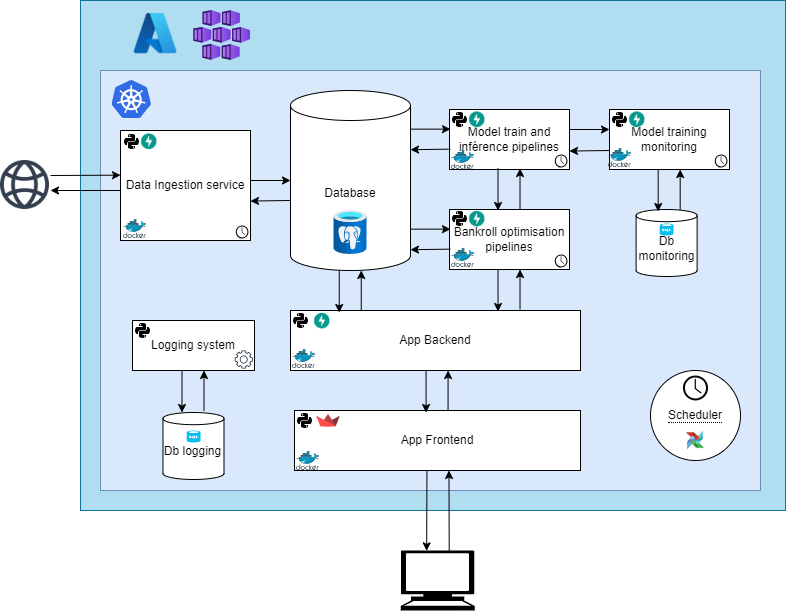
\includegraphics[width=0.8\textwidth, keepaspectratio]{images/diagrem_archi_services.png}
    \caption{Architecture of the system deployed on AKS}
    \label{fig:diagramme_arch_aks}
\end{figure}

\subsection{Infrastructure Details}

Our AKS deployment utilizes two virtual machines to ensure high availability and load balancing across the cluster. While Azure offers its own virtual machines, in this context, we refer to the compute resources allocated to our Kubernetes nodes. The integration with AKS allows for efficient resource utilization and scalability.

\subsection{Azure Services Integration}

Using Azure's cloud infrastructure offers several benefits:

\begin{itemize}
    \item \textbf{Azure Container Registry (ACR)}: Stores our Docker images securely, facilitating seamless deployment to AKS.
    \item \textbf{Azure DevOps Repo}: Provides a storage for our code.
\end{itemize}

\subsection{Pricing Considerations}

Azure's pricing model charges for compute resources used by virtual machines, storage, and network bandwidth. Managed services like AKS can reduce operational overhead but require careful monitoring to manage costs effectively. We optimized resource allocation by:


\section{Conclusion}

By adopting a microservices architecture, containerization with Docker, orchestration with Kubernetes, and deploying on Azure AKS, we built a scalable, reliable, and maintainable system for sports betting optimization. This architecture allows for independent development and deployment of components, ensuring the system can adapt to changing requirements and handle real-time data processing demands efficiently. Leveraging cloud infrastructure and managed services enhances our ability to focus on core application development while ensuring high availability and performance.
